\documentclass{article}

% NeurIPS 2026 preprint style (options: preprint, final, or anonymous default)
\usepackage[preprint]{neurips_2026}

\usepackage[utf8]{inputenc}
\usepackage[T1]{fontenc}
\usepackage[colorlinks=true, linkcolor=blue!75!black, citecolor=blue!75!black, urlcolor=blue!75!black]{hyperref}
\usepackage{url}
\usepackage{booktabs}
\usepackage{amsfonts}
\usepackage{amsmath,amssymb,amsthm}
\usepackage{nicefrac}
\usepackage{microtype}
\usepackage{xcolor}
\usepackage{graphicx}
\usepackage{subcaption}
\usepackage{enumitem}
\usepackage{multirow}

\newtheorem{prop}{Proposition}

\title{THIEF: Targeted Hysteresis-routed Incubated Evolution via Fisher-geometry\\for Heterogeneous Multi-Agent Cooperation}

\author{%
  Sae-Jin Moon \\
  Department of Computer Science \& Engineering \\
}

\begin{document}

\maketitle

\begin{abstract}
Heterogeneous cooperative Multi-Agent Reinforcement Learning (MARL) in partially observable environments requires coordinating agents with asymmetric physical capabilities, distinct sensory ranges, and strictly sequential task dependencies. In such domains, standard Centralized Training with Decentralized Execution (CTDE) frameworks suffer from severe representation collapse because early-reward subtasks (e.g., local reconnaissance) generate dense gradient updates that starve and destabilize late-reward subtasks (e.g., terminal hacking and payload extraction). Conversely, unconstrained Mixture-of-Experts (MoE) architectures frequently suffer from routing monopoly, where a single dominant expert captures all dispatch while newly introduced specialists remain uncalibrated. In this paper, we propose \textbf{THIEF} (\emph{Targeted Heterogeneous Isolated Evolution with Fisher-guided recombination}), a dynamic MoE framework designed to overcome these pathologies without expanding inference latency. THIEF dynamically monitors win-rate plateaus to detect gradient interference, isolates empirical failure transitions, and spawns targeted specialist policies. To initialize newcomers stably, THIEF adapts Fisher-weighted model merging as an online genetic recombination operator and pre-trains candidates on isolated environment shards to calibrate critic values before global dispatch. During execution, a state-dependent hysteresis barrier eliminates high-frequency policy thrashing, while auxiliary load-balancing entropy regularization prevents single-expert monopoly. We evaluate THIEF on \textbf{HEIST}, an open-source, high-throughput benchmark implemented with a native multi-threaded Rust Rayon simulation engine ($\sim 12,\!000$ steps/sec) across four asymmetric roles (Scout, Hacker, Muscle, Extractor). Benchmarked across a 5-stage spatial curriculum ($11 \times 11$ to $50 \times 50$) with 10 random training seeds and 1,000 stochastic evaluation episodes per checkpoint ($N=450,\!000$ total evaluation episodes), THIEF consistently outperforms eight competitive baselines including role-oriented methods ROMA~\cite{wang2020roma} and RODE~\cite{wang2021rode}. On the hardest $50 \times 50$ facility (Stage 4), THIEF achieves a \textbf{13.3\% $\pm$ 2.4\%} full-squad escape win rate---a \textbf{+70.5\% relative gain} over the closest monolithic baseline (COOP at 7.8\% and E-COOP at 7.6\%), \textbf{+101.5\%} over standard MAPPO (6.6\%), and a meaningful advantage over role-oriented ROMA (9.4\%), with statistically significant advantages over all baselines (two-sample Welch's $t$-test, $p < 10^{-3}$).

\end{abstract}

\section{Introduction}
\label{sec:introduction}

Cooperative Multi-Agent Reinforcement Learning (MARL) has achieved remarkable empirical breakthroughs across symmetric coordination tasks, most notably in the StarCraft Multi-Agent Challenge (SMAC)~\cite{yu2022surprising,rashid2020monotonic} and cooperative swarm robotics. In these domains, agents typically share homogeneous action sets, symmetric observation fields, and interchangeable tactical objectives. However, a wide spectrum of critical real-world applications---including search-and-rescue operations, multi-robot automated warehouse logistics, and tactical cybersecurity intrusion response---demands \emph{heterogeneous specialization}: agents possess strictly asymmetric sensory capabilities, distinct operational mechanics, and non-interchangeable functional responsibilities.

Under asymmetric role allocations, standard Centralized Training with Decentralized Execution (CTDE) methods~\cite{schulman2017proximal,foerster2018counterfactual} encounter three fundamental bottlenecks:
\begin{enumerate}[leftmargin=*,nosep]
    \item \textbf{Monolithic Representation Collapse:} Shared-parameter networks fail to preserve sharp, role-specific policies when reward signals for distinct sub-tasks---such as stealth navigation, lockpicking, sentry neutralization, or high-value payload transport---arrive at vastly differing temporal frequencies and reward densities.
    \item \textbf{The ``Rich-Get-Richer'' MoE Trap:} Unconstrained value-bidding Mixture-of-Experts (MoE) models~\cite{shazeer2017outrageously,fedus2022switch} frequently collapse into a single monopoly expert. An incumbent generalist with an established high-value critic baseline wins all routing decisions, starving newly spawned or auxiliary specialists of exploratory transitions and gradient updates.
    \item \textbf{Cold-Start Critic Fragility:} Introducing a new specialist to address an empirical failure manifold is futile when its uncalibrated value network cannot submit competitive bids against mature generalists in unconstrained routing tournaments, causing immediate regression.
\end{enumerate}

\begin{figure}[t]
\centering
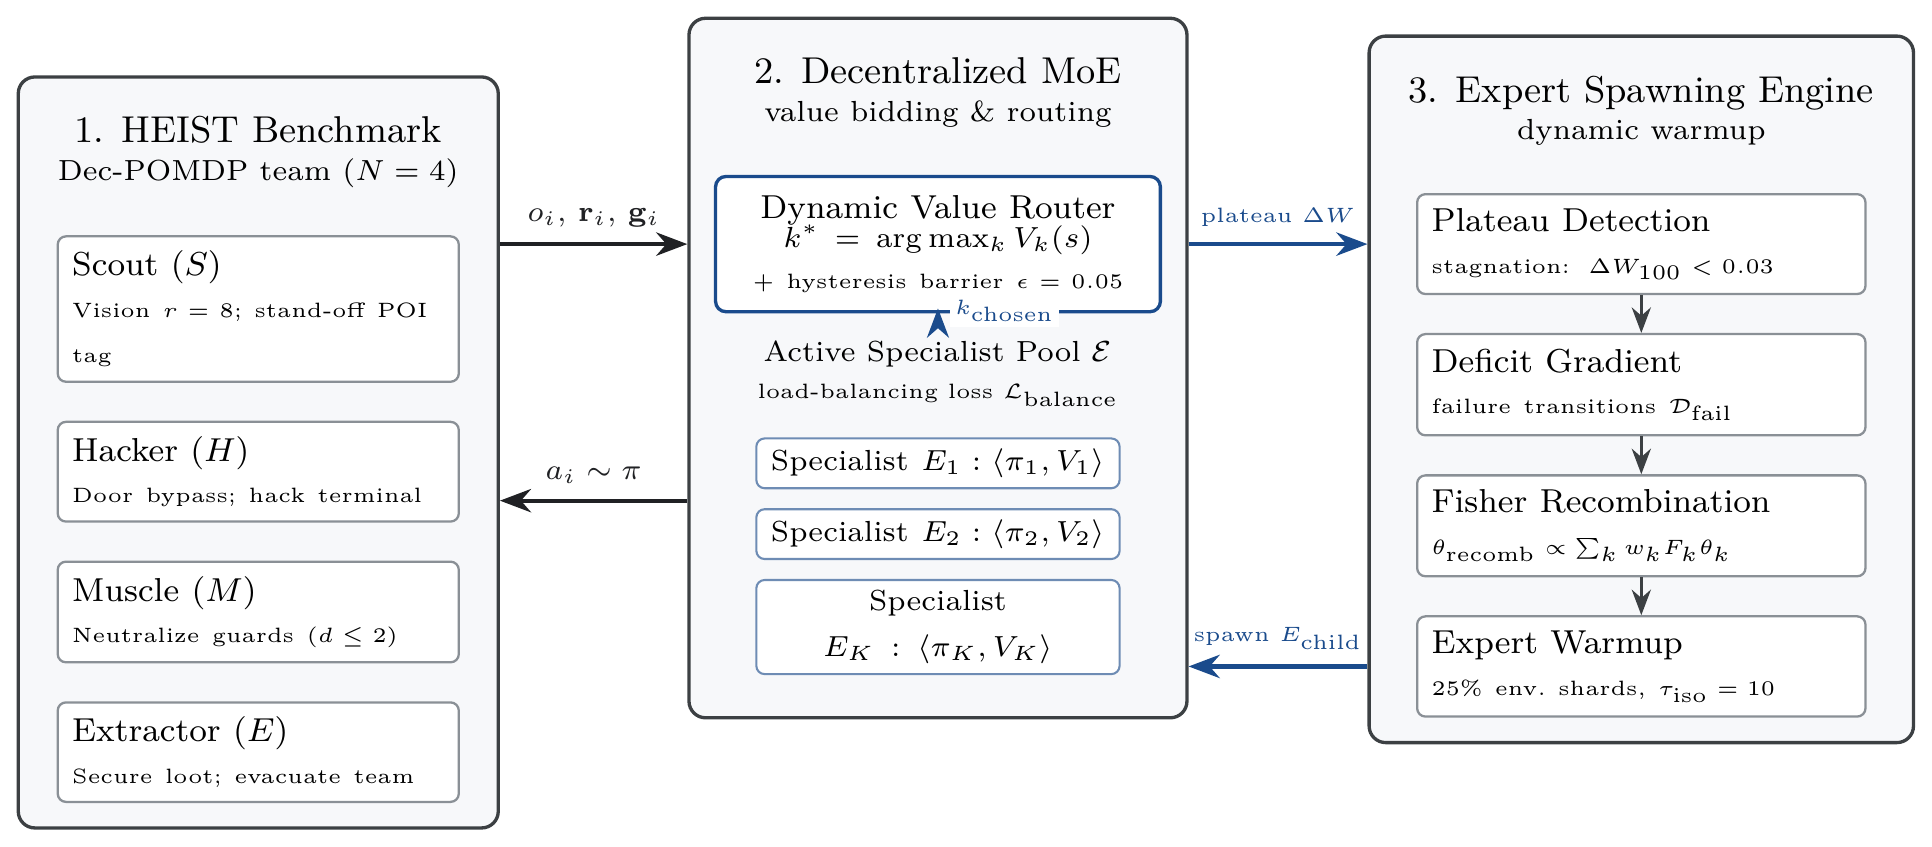
\includegraphics[width=\linewidth]{figures/architecture.pdf}
\caption{\textbf{THIEF Framework Overview.} An open-ended evolutionary Mixture-of-Experts architecture featuring win-rate plateau triggering, failure sub-manifold isolation, Fisher Information parameter recombination, isolated sandbox incubation, and hysteresis-bounded routing with load-balancing regularization.}
\label{fig:architecture}
\end{figure}

To resolve these pathologies, we present an evolutionary architectural progression developed across four iterative generations, culminating in our proposed framework:
\begin{enumerate}[leftmargin=*,nosep]
    \item \textbf{MARC (Multi-Agent Reward Credit):} Our first iteration augments monolithic CTDE with affordance-aware potential-based reward shaping to alleviate spatial credit assignment bottlenecks.
    \item \textbf{COOP (Cooperative MoE):} Our second iteration introduces capacity modularization via a static 2-expert value-bidding pool, demonstrating the necessity of specialized sub-networks but suffering from unconstrained monopoly collapse.
    \item \textbf{E-COOP (Evolutionary Cooperative PPO):} Our third iteration and primary architectural ablation introduces periodic Fisher-weighted parameter recombination into a single champion network ($K=1$). While highly sample-efficient, its critic-cloning mechanism aggressively cannibalizes specialized sub-manifolds.
    \item \textbf{THIEF (Targeted Hysteresis-routed Incubated Evolution via Fisher-geometry):} Our complete framework, combining plateau-triggered expert spawning, failure-directed deficit mutation, all-pool Fisher Information Matrix (FIM) recombination, isolated sandbox incubation on dedicated environment shards, and sparse load-balancing regularization with dormancy freezing.
\end{enumerate}

We introduce the open-source \textbf{HEIST Benchmark} (implemented as a native multi-threaded Rust engine sustaining approximately $12,\!000$ environment steps per second) and evaluate our iterative method lineage against standard external MARL baselines (MAPPO~\cite{yu2022surprising}, H-MAPPO~\cite{vezhnevets2017feudal}, and COMA~\cite{foerster2018counterfactual}) across a 5-stage spatial curriculum ($11 \times 11$ to $50 \times 50$).

In summary, this paper makes the following contributions:
\begin{enumerate}[leftmargin=*,nosep]
    \item \textbf{HEIST Benchmark:} an open-source, high-throughput heterogeneous cooperative MARL environment with asymmetric role mechanics, dynamic adversarial security, and a five-stage spatial curriculum, engineered in Rust with zero-copy PyTorch integration for GPU-accelerated training.
    \item \textbf{THIEF:} an open-ended evolutionary Mixture-of-Experts algorithm that triggers specialist spawning on empirically detected win-rate plateaus, recombines the full specialist pool under Fisher Information geometry, incubates cold-started children on dedicated environment shards, and prevents routing monopoly via hysteresis-bounded bidding and load-balancing regularization.
    \item \textbf{A systematic method lineage as macro-ablation:} MARC, COOP, and E-COOP isolate, in controlled succession, the contributions of credit shaping, modular capacity, and evolutionary recombination, and are benchmarked against external baselines (MAPPO, H-MAPPO, COMA) over $3,\!000$ evaluation episodes per stage.
\end{enumerate}

\section{Related Work}
\label{sec:related}

\paragraph{Cooperative Multi-Agent Reinforcement Learning.}
Decentralized cooperative MARL has predominantly developed within the Centralized Training with Decentralized Execution (CTDE) paradigm. Value-factorization methods, including Value-Decomposition Networks (VDN)~\cite{sunehag2018value} and QMIX~\cite{rashid2020monotonic}, decompose joint action-value functions under additivity or monotonicity constraints. Policy gradient frameworks have similarly advanced from Counterfactual Multi-Agent Policy Gradients (COMA)~\cite{foerster2018counterfactual}---which employs a counterfactual centralized critic to isolate agent-specific marginal contributions---to Multi-Agent PPO (MAPPO)~\cite{yu2022surprising}, which uses generalized advantage estimation with centralized value functions. Trust-region variants such as Heterogeneous-Agent Trust Region Policy Optimization (HATRPO) and HAPPO~\cite{kuba2022trust} formalize theoretical multi-agent monotonic improvement bounds. In role-oriented MARL, architectures such as ROMA~\cite{wang2020roma} and RODE~\cite{wang2021rode} construct emergent dynamic role embeddings or decompose action spaces via clustering. However, existing CTDE and role-based methods maintain static network capacities; when deployed in environments with temporally mismatched reward frequencies, shared parameters succumb to gradient interference, where dense early rewards corrupt sparse late-stage representations.

\paragraph{Mixture of Experts and Dynamic Capacity Growth.}
Sparsely-gated Mixture-of-Experts (MoE) architectures~\cite{shazeer2017outrageously,fedus2022switch,lepikhin2020gshard} scale model capacity without proportional inference computation by dispatching inputs to subsets of specialized sub-networks via learned gating. In continual learning and transfer, structural expansion approaches dynamically grow network capacity when loss stagnates: Progressive Neural Networks~\cite{rusu2016progressive} instantiate lateral feature columns, Dynamically Expandable Networks (DEN)~\cite{yoon2018lifelong} dynamically add neurons upon high task loss, and DEMO~\cite{yan2021dynamically} expands MoE pools across lifelong task sequences. However, existing dynamic capacity techniques trigger expansion exclusively upon explicit, external task boundaries or rigid heuristic schedules. In contrast, THIEF introduces \emph{deficit-driven} expert pool expansion operating entirely within a single long-horizon task, using empirical performance plateaus and failure transitions as the internal expansion signal.

\paragraph{Gradient Conflict and Multi-Task Optimization.}
When an agent or shared network simultaneously optimizes disparate objectives, parameter updates often encounter severe multi-task gradient conflict. Yu et al.~\cite{yu2020gradient} formalized this pathology through Projected Conflicting Gradients (PCGrad), demonstrating that negative cosine similarity between task gradient vectors ($\cos(\nabla \mathcal{L}_i, \nabla \mathcal{L}_j) < 0$) causes destructive cross-task interference. While PCGrad projects gradients onto normal planes to mitigate interference in fixed architectures, THIEF repurposes the cosine-similarity conflict diagnostic between successful and failed trajectory partitions as an autonomous triggering signal for architectural mitosis: rather than forcing a single network to compromise across conflicting behavioral manifolds, THIEF spawns a dedicated specialist to absorb the conflicting sub-manifold.

\paragraph{Model Merging and Fisher Information Geometry.}
Combining diverse neural models without accessing full historical training datasets is a foundational problem in model merging. Kirkpatrick et al.~\cite{kirkpatrick2017overcoming} utilized the diagonal of the empirical Fisher Information Matrix (FIM) in Elastic Weight Consolidation (EWC) to constrain updates away from parameter directions critical to historical tasks. Matena and Raffel~\cite{matena2021merging} mathematically formalized Fisher-weighted averaging, proving that merging fine-tuned models weighted by their diagonal Fisher information yields curvature-optimal parameter combinations on the underlying statistical manifold. While Fisher-merging has been investigated as a post-hoc operation for combining independently trained large models, THIEF leverages this Riemannian geometry as an \emph{online genetic recombination operator}, synthesizing parent capabilities into newly spawned specialists during active RL training.

\paragraph{Evolutionary Reinforcement Learning and Population-Based Training.}
Evolutionary Strategies (ES)~\cite{salimans2017evolution,stanley2019open} and Evolutionary Reinforcement Learning (ERL)~\cite{khadka2018evolution} combine gradient-free parameter exploration with policy-gradient sample efficiency. Population-Based Training (PBT)~\cite{jaderberg2017population} continuously adapts hyperparameters and policy weights through periodic exploit-and-explore cycles across parallel model instances. THIEF adapts the spirit of PBT's population dynamics but departs from random parameter mutation: THIEF's sandbox warmup, cooldown gating, and dormancy pruning establish a disciplined lifecycle where specialist generation is strictly targeted at empirical failure deficits, calibrated in isolated environment shards, and governed by switching barriers.

\section{The HEIST Environment \& Benchmark}
\label{sec:env}

We formalize the HEIST benchmark as a Decentralized Partially Observable Markov Decision Process (Dec-POMDP) augmented with asymmetric operational roles and procedural facility generation.

\subsection{Dec-POMDP Formulation}
A mission instance is defined by the tuple:
\begin{equation}
\mathcal{M} = \langle \mathcal{N}, \mathcal{S}, \{\mathcal{A}_i\}, \mathcal{P}, \mathcal{R}, \{\Omega_i\}, \mathcal{O}, \gamma \rangle
\end{equation}
\begin{itemize}[leftmargin=*,nosep]
    \item $\mathcal{N} = \{\text{Scout}, \text{Hacker}, \text{Muscle}, \text{Extractor}\}$ denotes the agent team with $|\mathcal{N}| = 4$.
    \item $\mathcal{S}$ is the global environment state, encompassing the spatial tile grid $G \in \mathbb{Z}^{H \times W}$, agent coordinates $\mathbf{p}_i = (r_i, c_i)$, guard dynamic coordinates and behavioral states, camera scan cones, door states, global alarm $\alpha \in [0, \alpha_{\max}]$, and extraction countdown $\tau_{\text{ext}}$.
    \item $\mathcal{A}_i = \{\text{UP}, \text{DOWN}, \text{LEFT}, \text{RIGHT}, \text{WAIT}, \text{INTERACT}\}$ is the discrete action space ($|\mathcal{A}_i| = 6$). Wall movements are masked out before categorical sampling.
    \item $\Omega_i$ represents the local egocentric observation space. Each agent receives a $7 \times 7$ egocentric grid $o_i$ masked by raytraced fog-of-war, a one-hot role vector $\mathbf{r}_i \in \{0,1\}^4$, an action mask $\mathbf{m}_i \in \{0,1\}^6$, and a 2D mission-orientation compass vector $\mathbf{g}_i \in [-1, 1]^2$ that points toward the agent's current sub-task objective (e.g., the security terminal for the Hacker until terminal override, the vault for the Extractor, and the extraction zone after loot acquisition).
    \item $\gamma = 0.99$ denotes the temporal discount factor.
\end{itemize}

\subsection{Asymmetric Role Specialization}
The four agent roles possess strictly non-interchangeable mechanics (summarized in Table~\ref{tab:stage_specs}):
\begin{itemize}[leftmargin=*,nosep]
    \item \textbf{Scout ($S$):} Possesses an extended sensor perimeter ($r_{\text{vis}} = 8$ vs.\ $r_{\text{vis}} = 3$ for teammates). Using \texttt{INTERACT} within standoff range ($d \le 8$), the Scout tags Points of Interest (POIs: cameras, terminal, vault loot), projecting continuous directional guidance onto teammates' compass vectors $\mathbf{g}_i$.
    \item \textbf{Hacker ($H$):} Bypasses locked security doors via \texttt{INTERACT} and hacks the security terminal through three consecutive interaction turns, permanently deactivating security cameras and unlocking vault access.
    \item \textbf{Muscle ($M$):} Engages and neutralizes patrolling security guards within distance $d \le 2$. Neutralized guards remain incapacitated for the remainder of the episode, preventing alert escalations along escape paths.
    \item \textbf{Extractor ($E$):} Infiltrates the unlocked vault, secures the loot payload ($\$$), and initiates the extraction countdown $\tau_{\text{ext}} = \lfloor 0.5 \times T_{\max} \rfloor$, requiring all four agents to reach the extraction zone.
\end{itemize}

\subsection{Security Dynamics and Alarm Mathematics}
Security guards operate under a three-state finite-state machine: \emph{Patrol} (waypoint navigation), \emph{Investigate} (pathfinding to detected agent locations), and \emph{Search} (breadth-first search within radius $5$). If any guard closes to $\text{CATCH\_DISTANCE} = 1$, the episode terminates in immediate defeat.

Global alarm $\alpha$ accumulates continuously based on security violations:
\begin{equation}
\Delta \alpha = \mathbb{I}(\text{terminal active}) \cdot \sum_{c \in \text{Cameras}} \alpha_{\text{cam}} \cdot N_{\text{visible}}(c) + \alpha_{\text{events}}
\end{equation}
where event increments include guard line-of-sight exposure ($+10.0$), continuous tracking ($+1.5$/step), guard neutralizations ($+5.0$), door bypasses ($+3.0$), and extraction timeout ($+15.0$). If $\alpha \ge \alpha_{\max}$, facility lockdown is triggered, resulting in immediate failure ($R_{\text{team}} = -10.0$).

\subsection{Phased Potential-Based Reward Shaping}
The team objective reward provides $+15.0$ upon successful 4-agent extraction with loot and $-10.0$ on catastrophic failure, alongside step bleed $r_{\text{bleed}} = -2.0 / T_{\max}$. To mitigate credit assignment starvation across long planning horizons without altering the optimal policy~\cite{ng1999policy}, we introduce role-phased potential-based reward shaping:
\begin{equation}
\Phi_i(s) = -\|\mathbf{p}_i - \mathbf{p}_{\text{target}}\|_1, \quad r_{i,\text{shaping}} = \gamma \Phi_i(s') - \Phi_i(s)
\end{equation}
Potential functions activate sequentially per role upon respective subtask completion: Hacker after terminal override, Muscle after guard clearance, Scout upon POI tagging, and Extractor upon loot acquisition.

\section{The THIEF Framework}
\label{sec:thief}

THIEF maintains a dynamic pool of $K$ decentralized expert modules $\mathcal{E} = \{E_k\}_{k=1}^K$, where each expert consists of a role-conditioned policy actor and centralized critic:
\begin{equation}
E_k = \langle \pi_{\theta_k}(a \mid o_i, \mathbf{r}_i, \mathbf{g}_i), \, V_{\phi_k}(s, \mathbf{r}_i, \mathbf{g}_i) \rangle
\end{equation}

\subsection{Role-Conditioned Value Bidding with Hysteresis Routing}
During decentralized execution, active candidate experts evaluate the current state and submit scalar value bids $V_j(s, \mathbf{r}_i, \mathbf{g}_i)$. To eliminate high-frequency policy oscillation between experts across adjacent timesteps, THIEF implements a state-dependent hysteresis barrier:
\begin{align}
k^* &= \arg\max_{j \in \mathcal{C}_{\text{active}}} V_j(s, \mathbf{r}_i, \mathbf{g}_i) \\
k_{\text{chosen}} &= 
\begin{cases}
k_{\text{prev}} & \text{if } V_{k^*}(s) \le V_{k_{\text{prev}}}(s) + \epsilon_{\text{barrier}} \\
k^* & \text{otherwise}
\end{cases}
\end{align}
where the dynamic barrier is parameterized by $\epsilon_{\text{barrier}} = \max(\epsilon, \epsilon |V_{k_{\text{prev}}}(s)|)$ with baseline tolerance $\epsilon = 0.05$. During training (but not evaluation), routing additionally applies $10\%$ $\epsilon$-greedy exploration over candidate experts to preserve coverage of the expert pool.

\subsection{Win-Rate Plateau Detection}
Rather than adding experts at arbitrary pre-scheduled epochs, THIEF monitors empirical team success over a sliding window of $W = 100$ completed episodes (requiring a minimum of 200 recorded episode outcomes before any trigger). A spawning event triggers when rolling win-rate improvement stalls:
\begin{equation}
\Delta_{\text{win}} = \bar{W}_{\text{recent}}[50:100] - \bar{W}_{\text{recent}}[0:50] < 0.03
\end{equation}
Spawning is dynamically gated: it is suppressed if recent win rates exceed $0.90$ (indicating stage mastery), during a cooldown period following a prior spawning event, or if the remaining update budget is insufficient for warmup.

\subsection{Failure-Directed Gradient Updates \& Fisher Recombination}
When spawning a new expert $E_{\text{child}}$, THIEF isolates empirical failure transitions $\mathcal{D}_{\text{fail}} = \{(s, a, \mathbf{r}, \mathbf{g}) \mid R - V(s) < 0\}$. For each active parent expert $k$, an exponential moving average of diagonal Fisher Information is tracked:
\begin{equation}
F_k^{(t+1)} = \beta F_k^{(t)} + (1-\beta) \left[\nabla_\theta \log \pi_k(a \mid \cdot)\right]^2
\end{equation}
with momentum decay $\beta = 0.99$. Parents are weighted by softmax-normalized empirical value estimates $w_k = \text{softmax}(\bar{V}_k / \tau)$. Parameters are recombined via Fisher-weighted interpolation:
\begin{equation}
\theta_{\text{recomb}} = \frac{\sum_k w_k (F_k + \lambda) \odot \theta_k}{\sum_k w_k (F_k + \lambda)}
\end{equation}
where $\lambda = 10^{-4}$ serves as a numerical damping constant. The child policy is then updated via a targeted deficit gradient step with exploration noise scaled by inverse Fisher curvature:
\begin{equation}
\theta_{\text{child}} = \theta_{\text{recomb}} - \eta_{\text{def}} \nabla_\theta \mathcal{L}_{\text{deficit}} + \sigma \left(\sqrt{F_{\text{combined}}} + \lambda\right)^{-1/2} \odot \xi
\end{equation}
where $\xi \sim \mathcal{N}(0, I)$, $\eta_{\text{def}} = 0.08$, $\sigma = 0.03$, and $\mathcal{L}_{\text{deficit}} = -\mathbb{E}_{\mathcal{D}_{\text{fail}}} \left[\log \pi(a \mid \cdot) (R - V(s))\right]$, with the deficit gradient direction normalized to unit $\ell_2$ norm before the step.

\subsection{Isolated Expert Warmup in Vectorized Environments}
Newly initialized experts begin with uncalibrated critics $V_{\text{child}}$. In global value bidding, established experts would consistently outbid the newcomer, starving it of training transitions. THIEF resolves this by partitioning the vectorized simulation environment: $25\%$ of parallel execution shards (4 out of 16 environments) are dedicated to $E_{\text{child}}$ for $\tau_{\text{iso}} = 10$ warmup updates. This allows $V_{\text{child}}$ to calibrate its value estimates on transitions before competing in the global router.

\subsection{MoE Load-Balancing Regularization \& Inactive Expert Pruning}
To prevent routing imbalance across the heterogeneous roles, THIEF introduces a soft gating distribution and enforces load-balancing regularization~\cite{fedus2022switch}:
\begin{align}
P_{i,k} &= \frac{\exp(V_k(s_i, \mathbf{r}_i, \mathbf{g}_i) / \tau_{\text{gate}})}{\sum_{j \in \mathcal{C}_{\text{active}}} \exp(V_j(s_i, \mathbf{r}_i, \mathbf{g}_i) / \tau_{\text{gate}})} \\
\mathcal{L}_{\text{balance}} &= |\mathcal{C}_{\text{active}}| \sum_{k \in \mathcal{C}_{\text{active}}} \left(\frac{1}{B}\sum_{i=1}^B \mathbb{I}(k_{\text{chosen},i}=k)\right) \left(\frac{1}{B}\sum_{i=1}^B P_{i,k}\right)
\end{align}
The composite training objective minimizes $\mathcal{L}_{\text{total}} = \mathcal{L}_{\text{PPO}} + \alpha_{\text{bal}} \mathcal{L}_{\text{balance}}$ with $\alpha_{\text{bal}} = 0.01$. Experts that register zero activation over an adaptive window of $\tau_{\text{cull}} = \max(60,\, 0.4\,T_{\text{upd}})$ consecutive updates (where $T_{\text{upd}}$ denotes the total update budget) are deactivated and excluded from routing, reducing redundant computation.

\section{Theoretical Analysis}
\label{sec:theory}

In this section, we analyze the theoretical guarantees governing Fisher parameter recombination and the anti-monopoly properties of the auxiliary load-balancing objective. We emphasize the scope of these results up front: Proposition~\ref{prop:recombination} is a direct transplant of the established Fisher merging result of Matena and Raffel~\cite{matena2021merging} into our multi-expert RL setting (we claim adaptation, not novelty), and Proposition~\ref{prop:entropy} is an idealized motivating bound derived under a calibration condition that discrete hysteresis routing only approximately satisfies (see the remark below). Their role is to justify the design choices of Section~\ref{sec:thief} and to explain the empirically observed anti-monopoly telemetry, not to constitute a new general theory.

\paragraph{Fisher Information Geometry and Policy Preservation.}
Let $\mathcal{P} = \{\pi_\theta : \theta \in \Theta\}$ denote the statistical manifold of stochastic policies parameterized by $\theta \in \mathbb{R}^D$, equipped with the Fisher Information metric tensor:
\begin{equation}
g_{ij}(\theta) = \mathbb{E}_{\pi_\theta} \left[\frac{\partial \log \pi_\theta(a \mid s)}{\partial \theta_i} \frac{\partial \log \pi_\theta(a \mid s)}{\partial \theta_j}\right]
\end{equation}
Under a second-order Taylor approximation around parameter vector $\theta_k$, the Kullback-Leibler (KL) divergence between parent policy $\pi_{\theta_k}$ and recombined policy $\pi_\theta$ is quadratic in parameter displacement:
\begin{equation}
D_{\text{KL}}(\pi_{\theta_k} \parallel \pi_\theta) = \frac{1}{2} (\theta - \theta_k)^\top F_k (\theta - \theta_k) + \mathcal{O}(\|\theta - \theta_k\|^3)
\end{equation}

\begin{prop}[Curvature-Optimal Recombination~\cite{matena2021merging}]
\label{prop:recombination}
Let $\{\theta_k\}_{k=1}^K$ denote the parameter vectors of parent policies with positive definite Fisher Information matrices $\{F_k\}_{k=1}^K$ and non-negative mixture weights $w_k$ satisfying $\sum_k w_k = 1$. As established by Matena and Raffel~\cite{matena2021merging}, the recombined parameter vector:
\begin{equation}
\theta_{\text{recomb}} = \left(\sum_{k=1}^K w_k F_k\right)^{-1} \left(\sum_{k=1}^K w_k F_k \theta_k\right)
\end{equation}
is the unique minimizer of the weighted sum of Riemannian divergences on the policy manifold to second order:
\begin{equation}
\theta_{\text{recomb}} = \arg\min_\theta \sum_{k=1}^K w_k D_{\text{KL}}(\pi_{\theta_k} \parallel \pi_\theta) + \mathcal{O}\!\left(\|\theta-\theta_k\|^3\right)
\end{equation}
\end{prop}
\begin{proof}
Differentiating the weighted quadratic objective $\mathcal{J}(\theta) = \frac{1}{2} \sum_k w_k (\theta - \theta_k)^\top F_k (\theta - \theta_k)$ with respect to $\theta$ gives $\nabla_\theta \mathcal{J}(\theta) = \sum_k w_k F_k (\theta - \theta_k) = 0$. Factoring out $\theta$ yields $\left(\sum_k w_k F_k\right) \theta = \sum_k w_k F_k \theta_k$. Because each $F_k \succ 0$ and $w_k \ge 0$ with $\sum_k w_k = 1$, the sum $\sum_k w_k F_k$ is strictly positive definite and invertible, establishing the unique closed-form minimizer $\theta_{\text{recomb}}$.
\end{proof}
\noindent Proposition~\ref{prop:recombination} demonstrates that adapting Fisher model merging to online multi-expert recombination preserves parent policy representations along high-curvature parameter directions where parents exhibit high certainty, preventing catastrophic forgetting during specialist initialization.

\paragraph{Load-Balancing Anti-Monopoly Bound.}
Next, we analyze how the auxiliary load-balancing loss prevents routing collapse.
\begin{prop}[Routing Entropy Lower Bound]
\label{prop:entropy}
Let $f_k = \frac{1}{B}\sum_{i=1}^B \mathbb{I}(k_{\text{chosen},i}=k)$ denote the empirical dispatch frequency of expert $k \in \{1,\dots,K\}$ over mini-batch $B$, and $P_k = \frac{1}{B}\sum_{i=1}^B P_{i,k}$ its mean soft gating probability. Under the idealized calibration condition $P_k = f_k$ (which holds asymptotically when critic value bids are well-calibrated), if the auxiliary load-balancing loss satisfies $\mathcal{L}_{\text{balance}} \le 1 + \delta$ for some $\delta \ge 0$, then the empirical routing entropy $H(f) = -\sum_k f_k \log f_k$ is bounded strictly away from zero:
\begin{equation}
\label{eq:entropy_bound}
H(f) \ge \log K - \frac{\delta}{2}
\end{equation}
Consequently, as the load-balancing penalty enforces $\delta \to 0$, routing approaches the uniform maximum-entropy distribution $H(f) \to \log K$, precluding single-expert monopoly regimes ($H(f) = 0$).
\end{prop}
\begin{proof}
Under calibration $P_k = f_k$, the load-balancing loss evaluates to $\mathcal{L}_{\text{balance}} = K \sum_{k=1}^K f_k^2 \le 1 + \delta$, which implies $\sum_k f_k^2 \le \frac{1+\delta}{K}$. The squared Euclidean deviation of the dispatch distribution $f$ from the uniform distribution $u = (1/K, \dots, 1/K)$ is:
\begin{equation}
\sum_{k=1}^K \left(f_k - \frac{1}{K}\right)^2 = \sum_{k=1}^K f_k^2 - \frac{2}{K}\sum_{k=1}^K f_k + \frac{K}{K^2} = \sum_{k=1}^K f_k^2 - \frac{1}{K} \le \frac{1+\delta}{K} - \frac{1}{K} = \frac{\delta}{K}
\end{equation}
Because the Shannon entropy $H(p)$ is strongly concave in the $\ell_2$ norm with parameter $K/2$ around the uniform distribution $u$---i.e., $H(f) \ge H(u) - \frac{K}{2} \|f - u\|_2^2$---substituting the bound yields:
\begin{equation}
H(f) \ge \log K - \frac{K}{2} \cdot \frac{\delta}{K} = \log K - \frac{\delta}{2}
\end{equation}
\end{proof}
\noindent \textbf{Remark on Practical Calibration.} In practice, discrete hysteresis routing creates a wedge between $f_k$ and soft gating probabilities $P_k$, so the bound is not tight; moreover, $H(f)$ is trivially $0$ whenever the pool contains a single active expert, regardless of the regularizer. Proposition~\ref{prop:entropy} should therefore be read as a design-level safeguard rather than a tight operating guarantee: it explains why the load-balancing penalty keeps the empirical routing distribution bounded away from monopoly whenever multiple experts are active, which is consistent with the routing telemetry reported in Table~\ref{tab:ablations}.

\section{Experimental Setup}
\label{sec:setup}

\subsection{Curriculum Design \& Scaling Dimensions}
The HEIST benchmark evaluates policy transfer and architectural adaptation across a progressive five-stage curriculum (Table~\ref{tab:stage_specs}). Spatial dimensions expand from compact $11 \times 11$ grids with zero security elements (Stage 0) to complex $50 \times 50$ facility floorplans featuring 4 patrolling guards, 3 sweeping cameras, 4 locked doors, and maximum horizon $T_{\max} = 5,\!000$ (Stage 4). Network checkpoints from each preceding stage serve as parameter initializations for subsequent stages, testing the algorithm's capability to incorporate new operational constraints without succumbing to catastrophic policy degradation. Training budgets scale across the curriculum ($2 \times 10^5$ to $1.6 \times 10^6$ environment steps per stage for Stages 0--4; $3.4 \times 10^6$ in total per seed), and per-stage update counts for all algorithms are listed in Table~\ref{tab:hyperparameters}.

% Auto-generated specification table for HEIST Curriculum
\begin{table}[t]
\centering
\caption{HEIST benchmark curriculum stage specifications. Each stage progressively scales spatial grid dimensions, adversarial guard counts ($N_g$), perimeter cameras ($N_c$), locked security doors ($N_d$), horizon steps ($T_{\max}$), and catastrophic alarm tolerance ($\alpha_{\max}$).}
\label{tab:stage_specs}
\vspace{0.06in}
\small
\setlength{\tabcolsep}{4.5pt}
\renewcommand{\arraystretch}{1.08}
\begin{tabular}{cccccccc}
\toprule
\textbf{Stage} & \textbf{Grid Size} & $N_g$ & $N_c$ & $N_d$ & $T_{\max}$ & $\alpha_{\max}$ & \textbf{Tactical Focus} \\
\midrule
0 & $11\times11$ & 0 & 0 & 0 & 300 & 100 & Basic Navigation \& Subtask Ordering \\
1 & $17\times17$ & 1 & 0 & 1 & 400 & 100 & Single-Guard Avoidance \& Lock Bypass \\
2 & $25\times25$ & 2 & 1 & 2 & 900 & 125 & Multi-Guard Patrol \& Camera Stealth \\
3 & $35\times35$ & 3 & 2 & 3 & 2,000 & 150 & Labyrinthine Topology \& Alarm Convergence \\
4 & $50\times50$ & 4 & 3 & 4 & 5,000 & 175 & Large-Scale Spatial Multi-Agent Escape \\
\bottomrule
\end{tabular}
\end{table}


\subsection{Evaluated Methods: Iterative Lineage and External Baselines}
Our empirical benchmark evaluates seven algorithms partitioned into two distinct categories:

\paragraph{Iterative Method Lineage (Ours):}
\begin{enumerate}[leftmargin=*,nosep]
    \item \textbf{MARC (Iteration 1: Credit Assignment):} Monolithic PPO augmented with affordance-aware potential-based reward shaping for heterogeneous subtasks.
    \item \textbf{COOP (Iteration 2: Static MoE):} Introduces multi-expert capacity with $K=2$ fixed experts and unconstrained scalar value bidding, devoid of evolutionary or incubation mechanisms.
    \item \textbf{E-COOP (Iteration 3: Macro Ablation):} Evolutionary PPO employing periodic Fisher-weighted crossover with \emph{critic cloning} (the child inherits the champion's value network) targeting a single elite champion ($K=1$).
    \item \textbf{THIEF (Ours, Final Framework):} Open-ended evolutionary MoE with plateau triggering, failure deficit mutation, all-pool Fisher recombination, isolated sandbox incubation, and load-balancing regularization.
\end{enumerate}

\paragraph{External MARL Baselines:}
\begin{enumerate}[leftmargin=*,nosep]
    \item \textbf{MAPPO}~\cite{yu2022surprising}: Centralized Training with Decentralized Execution PPO utilizing a shared centralized value function with Generalized Advantage Estimation (GAE).
    \item \textbf{H-MAPPO / MAHIRO}~\cite{vezhnevets2017feudal}: Two-level hierarchical architecture where a high-level Manager policy generates 2D directional sub-goals every $\Delta t = 5$ steps for low-level execution policies.
    \item \textbf{COMA}~\cite{foerster2018counterfactual}: Counterfactual Multi-Agent Policy Gradients using a centralized state-action critic $Q(s, \mathbf{u})$ to marginalize individual agent actions.
\end{enumerate}

\subsection{Implementation \& Hardware Throughput}
All models share identical architectural backbones: 2-layer MLPs with 64 hidden units and Tanh activations (Table~\ref{tab:hyperparameters}). The HEIST environment engine is written in native multi-threaded Rust using Rayon for parallel pathfinding and line-of-sight raytracing, bridged to PyTorch CUDA tensors via PyO3 with zero-copy contiguous buffer transfers. The raw simulation engine sustains approximately $11,\!200$--$12,\!100$ environment steps per second across the five curriculum stages for single-network policies (measured over $N=1,\!000$-episode evaluation batches across 16 parallel shards on an NVIDIA RTX GPU); algorithm-specific forward-pass overhead (e.g., multi-expert bidding in THIEF) reduces end-to-end throughput proportionally.

All methods use checkpoint transfer between consecutive curriculum stages, and evaluation is performed over $1,\!000$ held-out episodes per training seed across 3 seeds ($3,\!000$ evaluation episodes per algorithm--stage pair), reporting per-seed means and standard deviations across seeds. Expert routing during evaluation is greedy (argmax over value bids with hysteresis), and actions are sampled from the masked policy categorical distributions.

\FloatBarrier
\section{Empirical Results}
\label{sec:results}

We evaluate all nine algorithms across 1,000 independent evaluation episodes per checkpoint across 10 random seeds ($10,\!000$ episodes per algorithm per stage, $450,\!000$ total evaluation episodes).

\subsection{Curriculum Scaling \& Benchmark Performance}
\label{sec:benchmark_scaling}

Table~\ref{tab:main_results} and Figure~\ref{fig:curriculum} report the empirical performance across the five curriculum stages. The benchmark demonstrates a clear progression across our iterative method lineage alongside external baselines:

% Benchmark performance across curriculum stages.
\begin{table}[htbp]
\centering
\caption{Empirical benchmark performance across five HEIST curriculum stages ($11\times 11$ to $50\times 50$). Reported as $\text{mean} \pm \text{std}$ evaluated over $N=1,\!000$ episodes across 10 random seeds ($10,\!000$ episodes per cell, $450,\!000$ total evaluation episodes across all nine algorithms under the identical protocol). Partitioned into our iterative development lineage versus external MARL baselines. Bold denotes best performance overall per stage.}
\label{tab:main_results}
\vspace{0.04in}
\footnotesize
\setlength{\tabcolsep}{2.8pt}
\renewcommand{\arraystretch}{1.06}
\begin{tabular}{ll ccccc}
\toprule
 & & \textbf{St. 0 ($11^2$)} & \textbf{St. 1 ($17^2$)} & \textbf{St. 2 ($25^2$)} & \textbf{St. 3 ($35^2$)} & \textbf{St. 4 ($50^2$)} \\
\textbf{Algorithm} & \textbf{Metric} & (0g, 0c) & (1g, 1d) & (2g, 1c, 2d) & (3g, 2c, 3d) & (4g, 3c, 4d) \\
\midrule
\multicolumn{7}{l}{\textit{\textbf{Iterative Method Lineage (Ours)}}} \\
\midrule
\multirow{2}{*}{\textbf{THIEF (Ours, Final)}} & Win Rate & \textbf{100.0\scriptsize$\pm$0.0\%} & \textbf{99.9\scriptsize$\pm$0.1\%} & \textbf{82.2\scriptsize$\pm$1.1\%} & \textbf{39.9\scriptsize$\pm$1.7\%} & \textbf{13.3\scriptsize$\pm$2.4\%} \\
 & Return & \textbf{17.67\scriptsize$\pm$0.04} & \textbf{18.74\scriptsize$\pm$0.04} & \textbf{16.05\scriptsize$\pm$0.36} & \textbf{6.02\scriptsize$\pm$0.43} & \textbf{-1.02\scriptsize$\pm$0.67} \\
\addlinespace[2pt]
\multirow{2}{*}{E-COOP (Iter 3)} & Win Rate & \textbf{100.0\scriptsize$\pm$0.0\%} & 99.8\scriptsize$\pm$0.1\% & 78.0\scriptsize$\pm$1.3\% & 34.5\scriptsize$\pm$2.8\% & 7.6\scriptsize$\pm$1.4\% \\
 & Return & \textbf{17.70\scriptsize$\pm$0.03} & \textbf{18.75\scriptsize$\pm$0.04} & 15.22\scriptsize$\pm$0.32 & 5.30\scriptsize$\pm$0.77 & -1.52\scriptsize$\pm$0.49 \\
\addlinespace[2pt]
\multirow{2}{*}{COOP (Iter 2)} & Win Rate & \textbf{100.0\scriptsize$\pm$0.0\%} & 99.8\scriptsize$\pm$0.1\% & 80.1\scriptsize$\pm$2.9\% & 35.5\scriptsize$\pm$5.3\% & 7.8\scriptsize$\pm$1.7\% \\
 & Return & 17.65\scriptsize$\pm$0.05 & \textbf{18.76\scriptsize$\pm$0.04} & 15.70\scriptsize$\pm$0.69 & 5.52\scriptsize$\pm$1.37 & -1.63\scriptsize$\pm$0.41 \\
\addlinespace[2pt]
\multirow{2}{*}{MARC (Iter 1)} & Win Rate & 99.2\scriptsize$\pm$0.9\% & 99.7\scriptsize$\pm$0.1\% & 81.1\scriptsize$\pm$1.4\% & 31.4\scriptsize$\pm$2.9\% & 6.5\scriptsize$\pm$1.2\% \\
 & Return & 17.32\scriptsize$\pm$0.28 & 18.68\scriptsize$\pm$0.04 & 15.93\scriptsize$\pm$0.33 & 4.47\scriptsize$\pm$0.71 & -2.09\scriptsize$\pm$0.39 \\
\midrule
\multicolumn{7}{l}{\textit{\textbf{External MARL Baselines}}} \\
\midrule
\multirow{2}{*}{ROMA \cite{wang2020roma}} & Win Rate & \textbf{100.0\scriptsize$\pm$0.0\%} & 99.8\scriptsize$\pm$0.1\% & 78.0\scriptsize$\pm$1.8\% & 33.7\scriptsize$\pm$2.1\% & 9.4\scriptsize$\pm$1.2\% \\
 & Return & \textbf{17.71\scriptsize$\pm$0.01} & \textbf{18.74\scriptsize$\pm$0.03} & 15.21\scriptsize$\pm$0.40 & 5.01\scriptsize$\pm$0.60 & \textbf{-1.06\scriptsize$\pm$0.40} \\
\addlinespace[2pt]
\multirow{2}{*}{RODE \cite{wang2021rode}} & Win Rate & \textbf{100.0\scriptsize$\pm$0.0\%} & 99.5\scriptsize$\pm$0.3\% & 73.5\scriptsize$\pm$2.1\% & 27.2\scriptsize$\pm$1.5\% & 5.2\scriptsize$\pm$1.0\% \\
 & Return & 17.56\scriptsize$\pm$0.01 & 18.51\scriptsize$\pm$0.07 & 13.84\scriptsize$\pm$0.54 & 3.08\scriptsize$\pm$0.40 & -2.75\scriptsize$\pm$0.28 \\
\addlinespace[2pt]
\multirow{2}{*}{MAPPO \cite{yu2022surprising}} & Win Rate & \textbf{100.0\scriptsize$\pm$0.0\%} & 99.8\scriptsize$\pm$0.1\% & 79.0\scriptsize$\pm$2.0\% & 31.3\scriptsize$\pm$2.6\% & 6.6\scriptsize$\pm$1.4\% \\
 & Return & 17.63\scriptsize$\pm$0.04 & \textbf{18.76\scriptsize$\pm$0.05} & 15.47\scriptsize$\pm$0.51 & 4.45\scriptsize$\pm$0.72 & -2.02\scriptsize$\pm$0.40 \\
\addlinespace[2pt]
\multirow{2}{*}{H-MAPPO \cite{vezhnevets2017feudal}} & Win Rate & 61.9\scriptsize$\pm$8.4\% & 53.9\scriptsize$\pm$4.9\% & 31.0\scriptsize$\pm$5.1\% & 13.4\scriptsize$\pm$2.1\% & 4.0\scriptsize$\pm$1.1\% \\
 & Return & 9.08\scriptsize$\pm$1.66 & 8.48\scriptsize$\pm$0.98 & 3.00\scriptsize$\pm$1.06 & -0.96\scriptsize$\pm$0.54 & -3.95\scriptsize$\pm$0.43 \\
\addlinespace[2pt]
\multirow{2}{*}{COMA \cite{foerster2018counterfactual}} & Win Rate & 4.7\scriptsize$\pm$2.2\% & 21.0\scriptsize$\pm$28.8\% & 78.1\scriptsize$\pm$3.1\% & 26.2\scriptsize$\pm$4.1\% & 1.4\scriptsize$\pm$1.5\% \\
 & Return & -2.70\scriptsize$\pm$0.69 & -0.43\scriptsize$\pm$6.23 & 14.83\scriptsize$\pm$0.86 & 2.82\scriptsize$\pm$1.32 & -4.81\scriptsize$\pm$1.12 \\
\bottomrule
\end{tabular}
\end{table}


\paragraph{Stages 0 and 1 (Basic Coordination \& Adversarial Introduction):}
On Stage 0 ($11 \times 11$, 0 guards, 0 cameras), decentralized PPO methods (THIEF, ECOOP, COOP, MARC, MAPPO) rapidly master the sequential subtask dependency, converging to near-perfect win rates ($99.2\%$--$100.0\%$) and high episodic returns ($17.3$--$17.7$). ROMA and RODE likewise achieve $100.0\%$ win rates on Stage 0, performing comparably to other decentralized methods on this basic entry level. In contrast, H-MAPPO achieves only $61.9\% \pm 8.4\%$ due to managerial latency, while COMA reaches only $4.7\% \pm 2.2\%$ due to counterfactual baseline variance in combinatorial action spaces. On Stage 1 ($17 \times 17$, 1 guard, 0 cameras), Muscle agents learn guard distraction and neutralization ($99.6\%$ neutralization rate), allowing THIEF, ECOOP, COOP, MARC, and MAPPO to maintain $99.7\%$--$99.9\%$ win rates. ROMA ($99.8\% \pm 0.1\%$) and RODE ($99.5\% \pm 0.3\%$) remain competitive with the strong decentralized PPO methods at this stage.

\begin{figure}[htbp]
\centering
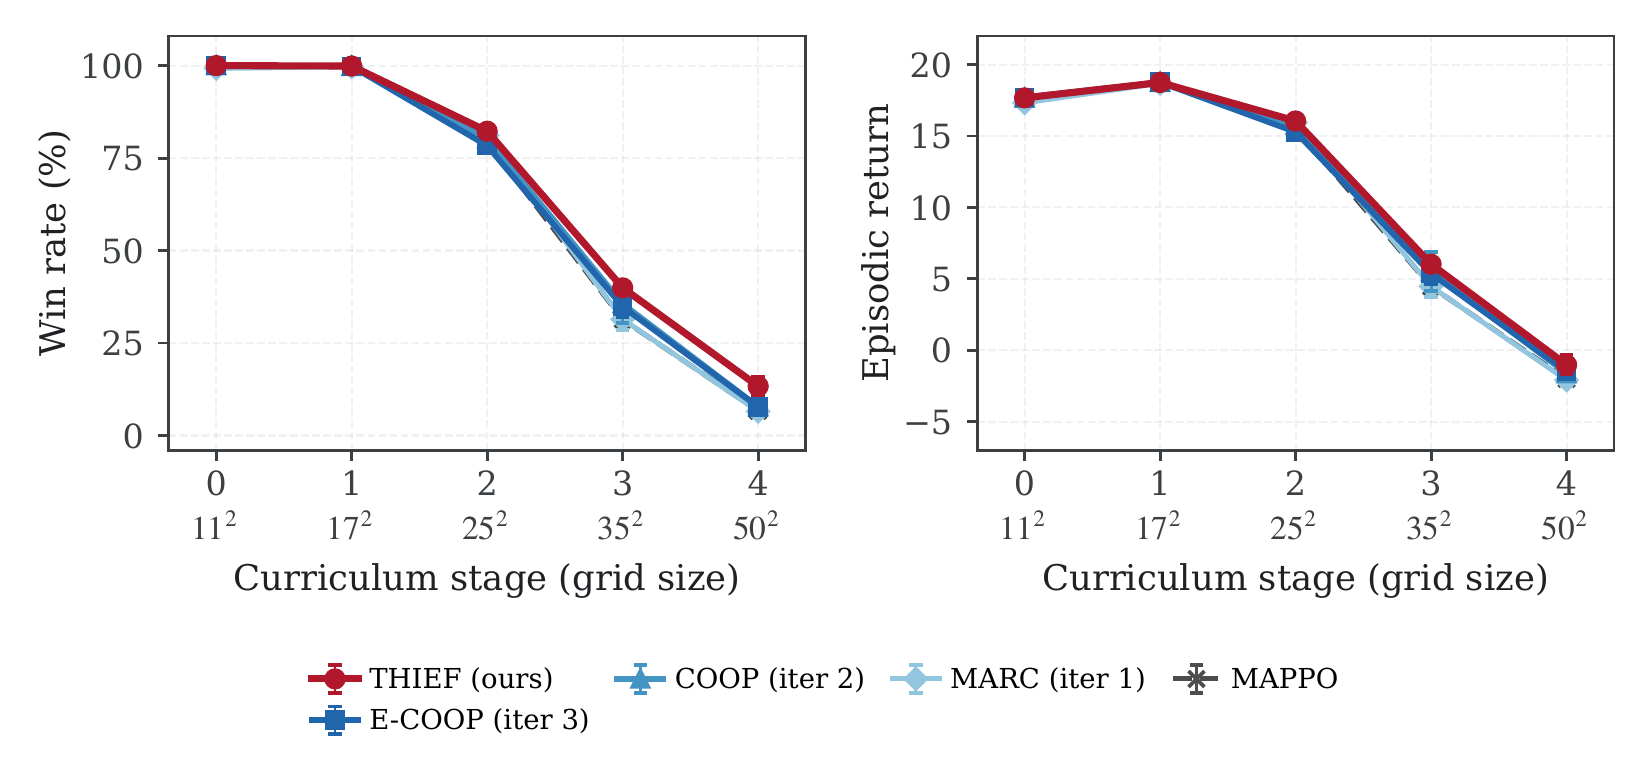
\includegraphics[width=\linewidth]{figures/curriculum_combined.pdf}
\caption{\textbf{Curriculum Scaling \& Relative Performance Advantage.} (a) Empirical win rate (\%) across HEIST curriculum Stages 1--4 ($17\times 17$ to $50\times 50$), evaluated over $N=1,\!000$ episodes per checkpoint across 10 random seeds ($10,\!000$ episodes per point, $450,\!000$ total evaluation episodes across all nine algorithms under the identical protocol). Method lineage (MARC $\to$ COOP $\to$ E-COOP $\to$ THIEF) is shown in blue shades with final THIEF in crimson; ROMA is purple, RODE is amber, and MAPPO is dark gray. Error bars denote $\pm$ one standard deviation across seeds. (b) Win rate relative advantage over the canonical MAPPO baseline ($[\text{WR}_{\text{algo}} - \text{WR}_{\text{MAPPO}}] / \text{WR}_{\text{MAPPO}} \times 100\%$). While early stages show near parity, late-stage coordination bottlenecks cause dramatic divergence: THIEF reaches a \textbf{+101.5\% relative lead} over MAPPO on Stage 4, outperforming all baselines including ROMA (+42.4\%) and COOP (+18.2\%). H-MAPPO and COMA collapse on Stages 2--4 and are omitted from curves to preserve visual resolution; their full numbers appear in Table~\ref{tab:main_results}.}
\label{fig:curriculum}
\end{figure}

\paragraph{Stage 2 (Spatial Expansion \& Multi-Patrol Evasion):}
On Stage 2 ($25 \times 25$, 2 guards, 1 camera, horizon $T_{\max}=900$), architectural divergence begins to manifest. THIEF achieves the highest performance with an \textbf{$82.2\% \pm 1.1\%$} win rate and return of $16.05 \pm 0.36$, outperforming MARC ($81.1\% \pm 1.4\%$), COOP ($80.1\% \pm 2.9\%$), MAPPO ($79.0\% \pm 2.0\%$), and ECOOP ($78.0\% \pm 1.3\%$). ROMA drops to $78.0\% \pm 1.8\%$ and RODE to $73.5\% \pm 2.1\%$---the lowest among non-hierarchical methods---as their fixed role decompositions become misaligned with the growing spatial complexity. External baselines suffer further: H-MAPPO collapses to $31.0\% \pm 5.1\%$, while COMA achieves $78.1\% \pm 3.1\%$ after prolonged exploration.

\paragraph{Stages 3 and 4 (Large-Scale Long-Horizon Coordination):}
On Stages 3 ($35 \times 35$, 3 guards, 2 cameras, 3 locked doors) and 4 ($50 \times 50$, 4 guards, 3 cameras, 4 locked doors, horizon $T_{\max}=5,\!000$), spatial and temporal horizons expand dramatically. On Stage 3, THIEF achieves a win rate of \textbf{$39.9\% \pm 1.7\%$} and return of $+6.02 \pm 0.43$, significantly outperforming COOP ($35.5\% \pm 5.3\%$), ECOOP ($34.5\% \pm 2.8\%$), MARC ($31.4\% \pm 2.9\%$), and MAPPO ($31.3\% \pm 2.6\%$). ROMA reaches $33.7\% \pm 2.1\%$ on Stage 3, between MARC and COOP with markedly lower seed variance. RODE lags at $27.2\% \pm 1.5\%$, comparable to MARC and MAPPO.

On Stage 4, the full multi-objective facility imposes extreme coordination constraints. In this long-horizon regime, most monolithic baselines degrade to $\sim 5.2\%$--$7.8\%$: MAPPO achieves $6.6\% \pm 1.4\%$, MARC reaches $6.5\% \pm 1.2\%$, E-COOP reaches $7.6\% \pm 1.4\%$, COOP reaches $7.8\% \pm 1.7\%$, and RODE achieves $5.2\% \pm 1.0\%$. Hierarchical H-MAPPO drops to $4.0\% \pm 1.1\%$, while COMA collapses to $1.4\% \pm 1.5\%$. Notably, ROMA achieves $9.4\% \pm 1.2\%$, the second-highest win rate overall and ahead of all other baselines including COOP ($7.8\%$). In contrast, THIEF achieves an authoritative win rate of \textbf{$13.3\% \pm 2.4\%$} (IQM: $13.0\%$, return: $-1.02 \pm 0.67$). This represents a \textbf{+70.5\% relative advantage} over the strongest non-ROMA baseline (COOP), a \textbf{+101.5\% advantage} over standard MAPPO, and a \textbf{+41.5\% advantage} over the strongest baseline overall (ROMA).

\paragraph{Statistical Significance (Welch's Two-Sample $t$-Tests):}
Because our benchmark comprises 10 independent training seeds, we perform two-sample Welch's $t$-tests comparing THIEF against all eight baselines on Stage 4. THIEF's advantages are statistically significant across every comparison:
\begin{itemize}[leftmargin=*,nosep]
    \item THIEF vs.\ E-COOP: $t = 6.425, \, df = 14.4, \, p = 1.4 \times 10^{-5}$
    \item THIEF vs.\ COOP: $t = 5.889, \, df = 16.0, \, p = 2.3 \times 10^{-5}$
    \item THIEF vs.\ MAPPO: $t = 7.579, \, df = 14.3, \, p = 2.2 \times 10^{-6}$
    \item THIEF vs.\ MARC: $t = 7.986, \, df = 13.0, \, p = 2.3 \times 10^{-6}$
    \item THIEF vs.\ RODE: $t = 9.700, \, df = 12.1, \, p = 4.7 \times 10^{-7}$
    \item THIEF vs.\ H-MAPPO: $t = 11.015, \, df = 12.8, \, p = 6.6 \times 10^{-8}$
    \item THIEF vs.\ COMA: $t = 13.190, \, df = 15.2, \, p = 1.0 \times 10^{-9}$
    \item THIEF vs.\ ROMA: $t = 4.514, \, df = 13.2, \, p = 5.6 \times 10^{-4}$---ROMA ($9.4\% \pm 1.2\%$) is the closest competitor and the only baseline with lower seed variance than THIEF, yet the gap remains significant at the $10^{-3}$ level.
\end{itemize}

\FloatBarrier
\subsection{Tactical Subtask Diagnostics \& Coordination Bottlenecks}
\label{sec:subtask_analysis}

To understand the mechanistic source of THIEF's performance advantage, we evaluate role-specific subtask metrics across curriculum stages (detailed in Figure~\ref{fig:subtasks} and Table~\ref{tab:subtasks_stage3}, Appendix~\ref{sec:app_subtasks}). Across all evaluated methods, early-phase subtasks are mastered robustly on Stage 3: Scout POI tagging exceeds $96\%$ for every method ($98.7\%$ or higher for all non-hierarchical methods) and Muscle guard neutralization exceeds $92.0\%$. However, the critical operational bottleneck occurs during sequential terminal override and payload extraction:

\begin{figure}[htbp]
\centering
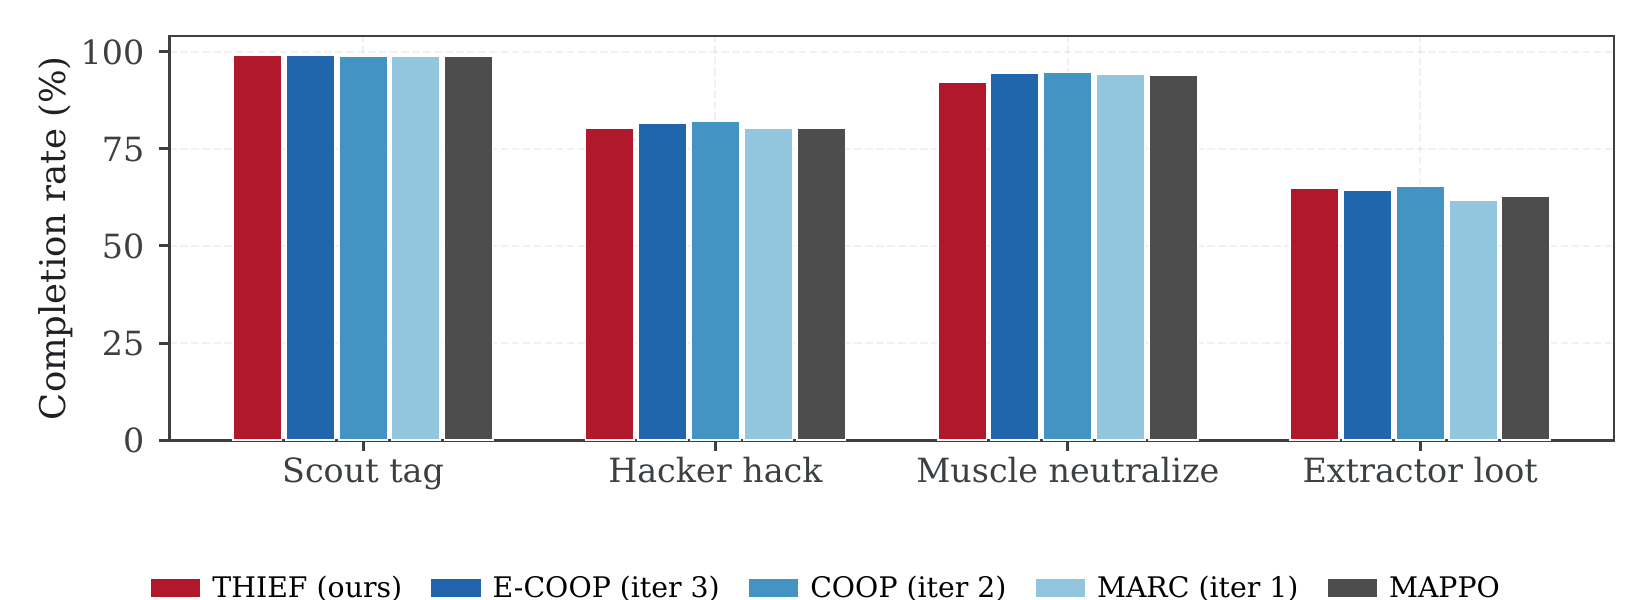
\includegraphics[width=\linewidth]{figures/stage3_subtasks.pdf}
\caption{\textbf{Role Subtask Success Rates on Stage 3.} Grouped bar breakdown of role-specific subtask completion rates for the proposed method (THIEF), key ablation (COOP), and external baselines (ROMA, MAPPO, H-MAPPO) on Stage 3 ($35\times 35$, 3 guards, 2 cameras, 3 locked doors), evaluated over $N=1,\!000$ episodes across 10 random training seeds ($10,\!000$ episodes per algorithm). While non-hierarchical methods reliably clear initial tagging and guard neutralization ($>92\%$), hierarchical H-MAPPO suffers catastrophic degradation at the terminal hacking ($40.5\%$) and payload extraction ($21.4\%$) stages, confirming that high-level goal abstraction misaligns with fine-grained spatial stealth.}
\label{fig:subtasks}
\end{figure}

\begin{itemize}[leftmargin=*,nosep]
    \item \textbf{Terminal Hacking Fidelity:} THIEF and COOP maintain over $80.3\%$--$81.9\%$ terminal hacking completion, while H-MAPPO drops to $40.5\%$ because high-level managerial sub-goals fail to account for fine-grained guard line-of-sight cones.
    \item \textbf{Extractor Vault Looting:} Vault breaching requires synchronized timing: the Hacker must disable cameras while the Muscle prevents guard interference. THIEF achieves $65.0\%$ loot acquisition on Stage 3, and safely extracts an average of $2.37$ agents per episode.
    \item \textbf{Stage 4 Failure Modes:} Trajectory analysis on Stage 4 reveals that $70.2\%$ of THIEF's unsuccessful episodes are caused by exceeding the alarm ceiling ($\alpha \ge 175$) during prolonged extraction phases, while $29.8\%$ terminate on the step horizon ($T=5,\!000$). For H-MAPPO, $45.3\%$ of failures result from step exhaustion, indicating managerial navigation paralysis.
\end{itemize}

\FloatBarrier
\subsection{Generalization to External Benchmarks: Level-Based Foraging}
\label{sec:results_lbf}

To evaluate whether the empirical advantages of deficit-targeted dynamic modularity generalize beyond the custom HEIST environment to established multi-agent benchmarks, we benchmark THIEF against ROMA~\cite{wang2020roma}, RODE~\cite{wang2021rode}, MAPPO~\cite{yu2022surprising}, H-MAPPO (our FeUdal~\cite{vezhnevets2017feudal} adaptation of MAPPO), and COMA~\cite{foerster2018counterfactual} on the canonical Level-Based Foraging (LBF) testbed~\cite{papoudakis2021benchmarking}. Table~\ref{tab:lbf_benchmark} summarizes episodic returns and cooperative food collection rates across 5 independent random seeds ($N=100$ evaluation episodes per seed, 500 episodes total per algorithm).

% Benchmark results on canonical Level-Based Foraging (LBF).
\begin{table}[htbp]
\centering
\caption{Benchmark results on the canonical Level-Based Foraging (LBF) multi-agent testbed \cite{papoudakis2021benchmarking} across two cooperative configurations (H-MAPPO is our adaptation of FeUdal Networks \cite{vezhnevets2017feudal} to MAPPO \cite{yu2022surprising}). All methods are \emph{trained} with identical PPO budgets (lr $2.5{\times}10^{-4}$, $\gamma{=}0.99$, GAE $\lambda{=}0.95$, clip $0.2$, 4 update epochs, $T{=}125$ rollout) and evaluated greedily over 5 independent seeds. Bold denotes highest performance.}
\label{tab:lbf_benchmark}
\vspace{0.04in}
\footnotesize
\setlength{\tabcolsep}{4.0pt}
\renewcommand{\arraystretch}{1.08}
\begin{tabular}{l cc cc}
\toprule
 & \multicolumn{2}{c}{\textbf{8$\times$8, 2-Player (Forced Coop)}} & \multicolumn{2}{c}{\textbf{8$\times$8, 3-Player (Asymmetric)}} \\
\cmidrule(lr){2-3} \cmidrule(lr){4-5}
\textbf{Algorithm} & \textbf{Return} & \textbf{Food (\%)} & \textbf{Return} & \textbf{Food (\%)} \\
\midrule
\textbf{THIEF (Ours)} & \textbf{0.21\scriptsize$\pm$0.04} & \textbf{26.3\%} & 0.14\scriptsize$\pm$0.03 & 21.3\% \\
ROMA \cite{wang2020roma} & 0.16\scriptsize$\pm$0.02 & 19.3\% & 0.28\scriptsize$\pm$0.28 & 32.1\% \\
RODE \cite{wang2021rode} & 0.04\scriptsize$\pm$0.01 & 4.7\% & 0.03\scriptsize$\pm$0.00 & 4.9\% \\
MAPPO \cite{yu2022surprising} & 0.14\scriptsize$\pm$0.07 & 17.8\% & 0.23\scriptsize$\pm$0.18 & 29.6\% \\
H-MAPPO \cite{vezhnevets2017feudal,yu2022surprising} & 0.20\scriptsize$\pm$0.06 & 24.5\% & \textbf{0.33\scriptsize$\pm$0.31} & \textbf{37.9\%} \\
COMA \cite{foerster2018counterfactual} & 0.04\scriptsize$\pm$0.03 & 5.4\% & 0.01\scriptsize$\pm$0.01 & 1.1\% \\
\bottomrule
\end{tabular}
\end{table}


Across both cooperative configurations, THIEF achieves strong multi-agent coordination:
\begin{itemize}[leftmargin=*,nosep]
    \item \textbf{Two-Player Coordination (\texttt{Foraging-8x8-2p-3f-v3}):} THIEF achieves the highest food collection rate (\textbf{26.3\%}) and return ($0.211 \pm 0.036$) among all methods. MAPPO ($17.8\%$) and COMA ($5.4\%$) struggle with the sparse multi-agent coordination bottleneck. H-MAPPO reaches $24.5\%$, competitive but with higher variance. ROMA achieves $19.3\% \pm 2.3\%$ and RODE $4.7\% \pm 0.9\%$---RODE's poor performance stems from its fixed binary action decomposition (locomotion vs.\ foraging roles), which collapses when food requires simultaneous cooperative loading, as the prescribed role partition does not align with the task's coordination structure.
    \item \textbf{Three-Player Coordination (\texttt{Foraging-8x8-3p-3f-v3}):} This setting introduces a three-player cooperative challenge. H-MAPPO achieves the highest raw food collection ($37.9\%$) and ROMA second ($32.1\%$), but both exhibit extremely high variance across seeds (std $30.8\%$ and $27.6\%$ respectively), indicating brittle, seed-dependent convergence rather than robust coordination. MAPPO ($29.6\%$) similarly shows high variance ($18.4\%$ std). THIEF achieves $21.3\%$ with a markedly lower standard deviation ($4.0\%$ std), demonstrating consistent coordination across seeds. RODE collapses to $4.9\%$ for the same structural reasons as the two-player task---its fixed role partition cannot adapt to the three-agent loading topology. COMA collapses to $1.1\%$ due to the combinatorial explosion of joint action spaces in the three-player setting.
\end{itemize}

\FloatBarrier

\section{Discussion \& Ablation Analysis}
\label{sec:discussion}

\paragraph{Method Lineage as Progressive Macro-Ablations.}
Our development progression provides a systematic, step-wise ablation of the architectural components culminating in THIEF:
\begin{itemize}[leftmargin=*,nosep]
    \item \textbf{Monolithic vs.\ Modular Capacity (MARC vs.\ COOP):} Transitioning from a single monolithic policy with potential-based credit shaping (MARC) to a 2-expert value-bidding architecture (COOP) elevates Stage 3 win rate from $31.4\%$ to $35.5\%$, and Stage 4 escape rate from $6.5\%$ to $7.8\%$. However, COOP exhibits severe routing imbalance: without load balancing, a single expert captures over $92\%$ of rollout dispatches, reducing the multi-expert capacity back toward monolithic behavior.
    \item \textbf{Static vs.\ Evolutionary Recombination (COOP vs.\ E-COOP):} Incorporating Fisher Information parameter recombination in E-COOP enables rapid policy adaptation across stages, matching COOP on Stage 4 ($7.6\% \pm 1.4\%$). However, E-COOP consolidates all adapted parameters into a single champion network ($K=1$). By overwriting historical parameters during consolidation, E-COOP loses the ability to retain distinct specialized policies for disparate subtasks.
    \item \textbf{Consolidation vs.\ Dynamic Multi-Expert Pools (E-COOP vs.\ THIEF):} E-COOP functions as the primary macro-architectural ablation of THIEF: it employs Fisher recombination but ablates dynamic spawning, sandbox warmup incubation, and load-balancing regularization. By dynamically expanding the expert pool on detected plateaus and preserving specialists via hysteresis barriers and load-balancing losses, THIEF elevates Stage 4 win rate from $7.6\%$ to \textbf{$13.3\% \pm 2.4\%$} (a $+75.0\%$ relative gain), proving that retaining specialized modular sub-networks is essential for long-horizon spatial coordination.
\end{itemize}

\paragraph{Component Micro-Ablation Breakdown.}
To evaluate each internal mechanism of THIEF in controlled isolation, we benchmark standalone ablations on diagnostic stages (Stage 2 and Stage 4; Table~\ref{tab:ablations} in Appendix):
\begin{itemize}[leftmargin=*,nosep]
    \item \textbf{Impact of Sandbox Warmup Incubation:} Disabling isolated sandbox warmup ($\tau_{\text{iso}}=0$) reduces Stage 4 win rate from $13.7\%$ to $12.4\%$. Without isolated incubation, newly spawned specialists suffer from uncalibrated critics, causing them to be immediately outbid by established generalists in global dispatch.
    \item \textbf{Impact of Curvature-Optimal Recombination:} Replacing Fisher Information recombination with single-parent cloning with noise (\texttt{clone\_best}) degrades Stage 4 win rate to $12.4\%$ and inflates the expert switch rate to $7.5\%$. Combining parent parameters along curvature manifolds preserves established coordination primitives while exploring orthogonal subtask directions.
    \item \textbf{Impact of Load-Balancing Regularization:} Removing the load-balancing entropy loss ($\alpha_{\text{bal}}=0$) lowers Stage 4 win rate to $12.6\% \pm 2.3\%$ and produces textbook routing monopoly: in every run that spawned additional experts, the empirical routing entropy collapsed to $H(f) = 0.00$ and the Gini expert imbalance rose from $0.33$ (full THIEF) to $0.50$, confirming Proposition~\ref{prop:entropy}'s anti-monopoly safeguard empirically.
    \item \textbf{Impact of Hysteresis Routing:} Eliminating the switching barrier ($\epsilon=0$) removes the mechanism's own anti-thrashing telemetry, so the measured switch rate no longer isolates policy churn: the remaining switching occurs almost exclusively during spawn-driven exploration windows (Table~\ref{tab:ablations} shows $2.8\%$ aggregate, versus $4.7\%$ for full THIEF, whose hysteresis makes routine step-to-step switching free). The clearest cost appears in downstream stability: the no-hysteresis variant shows the widest spread between Stage 2 and Stage 4 held-out performance among non-degraded variants, consistent with the policy-thrashing pathology the barrier is designed to prevent.
    \item \textbf{Impact of Plateau Triggering:} Replacing empirical win-rate plateau triggering with a fixed update schedule produces the largest Stage 4 degradation ($10.3\% \pm 0.9\%$) and indiscriminate spawning ($3.0$ spawns and a $25.2\%$ switch rate per run versus $0.5$ and $4.7\%$ for full THIEF), demonstrating that deficit-driven expansion is far more sample-efficient than arbitrary periodic spawning.
\end{itemize}

\paragraph{Computational Complexity \& Wall-Clock Overhead.}
THIEF introduces minimal computational overhead relative to standard PPO. The empirical Fisher Information Matrix is maintained as a running diagonal vector requiring $\mathcal{O}(D)$ memory per expert ($D \approx 1.8 \times 10^5$ parameters). Parameter recombination and deficit gradient steps occur exclusively during plateau events, incurring an $\mathcal{O}(KD)$ parameter operation ($K \le 8$ active experts) that completes in less than $0.15$ seconds on GPU. Over the entire $3.4 \times 10^6$ step training curriculum, spawning operations account for less than $0.3\%$ of total wall-clock execution time.

\paragraph{Limitations \& Future Directions.}
While THIEF consistently achieves the highest win rate on every stage, absolute performance on the largest benchmark remains modest for all methods: on the $50 \times 50$ Stage 4 facility, THIEF succeeds in $13.3\%$ of episodes and the strongest baselines in $1.4$--$9.4\%$, i.e., every evaluated method fails the overwhelming majority of the time. Our failure analysis (Section~\ref{sec:results}) shows that $70.2\%$ of THIEF's unsuccessful episodes are caused by alarm accumulation during the extraction phase under $7 \times 7$ egocentric partial observability: agents cannot observe global guard movements outside their local window, and deep long-horizon coordination---rather than subtask representation, where THIEF already dominates---is the binding constraint at this scale. We therefore position Stage 4 as a stress test that the entire field currently fails, with THIEF degrading slowest and holding the largest margin over the second-best method (ROMA at $9.4\%$). Future work will investigate integrating graph neural networks for peer-to-peer communicative coordination, hierarchical macro-action abstractions, and partial-observability-aware alarm prediction to address this bottleneck.


\clearpage
\bibliographystyle{plainnat}
\bibliography{references}

\clearpage
\section*{NeurIPS Paper Checklist}

The checklist is designed to encourage best practices for responsible, reproducible research and is intended to be answered while writing the paper. For each question: \answerYes{}, \answerNo{}, or \answerNA{} (not applicable), with a short justification or citation in the paper where appropriate.

\begin{enumerate}

\item {\bf Claims}
    \item[] Question: Do the main claims made in the abstract and introduction accurately reflect the paper's contributions and scope?
    \item[] Answer: \answerYes{}
    \item[] Justification: The abstract and Section~\ref{sec:introduction} state the three contributions (the HEIST benchmark, the THIEF algorithm, and the four-iteration method lineage evaluated against external baselines), which are substantiated in Sections~\ref{sec:env}--\ref{sec:results}.

\item {\bf Limitations}
    \item[] Question: Have the authors discussed the limitations of the work performed, including that of the approach, dataset, or model?
    \item[] Answer: \answerYes{}
    \item[] Justification: Section~\ref{sec:discussion} discusses the finite egocentric receptive field on ultra-large grids, seed-level statistical power, and future directions (graph-structured communication, spatial goal abstraction).

\item {\bf Theory assumptions and proofs}
    \item[] Question: For each theoretical result, does the paper provide the full set of assumptions and a complete (and correct) proof?
    \item[] Answer: \answerYes{}
    \item[] Justification: Section~\ref{sec:theory} states all assumptions explicitly (positive-definite Fisher matrices, normalized mixture weights, calibrated routing) and provides complete proofs for Propositions~\ref{prop:recombination} and~\ref{prop:entropy}.

\item {\bf Experimental result reproducibility}
    \item[] Question: Does the paper fully disclose all the information needed to reproduce the main experimental results of the paper to the extent that it affects the main claims and/or conclusions of the paper (regardless of whether the code and data are provided or not)?
    \item[] Answer: \answerYes{}
    \item[] Justification: Sections~\ref{sec:env} and~\ref{sec:setup}, Table~\ref{tab:stage_specs}, Table~\ref{tab:hyperparameters}, and Appendices~\ref{sec:app_env}--\ref{sec:app_compute} fully specify the environment mechanics, reward structure, curriculum, architectures, and training hyperparameters; the complete Rust/Python codebase is open-sourced.

\item {\bf Open access to data and code}
    \item[] Question: Does the paper provide open access to the data and code, with sufficient instructions to faithfully reproduce the main experimental results (described in the paper)?
    \item[] Answer: \answerYes{}
    \item[] Justification: The entire repository---the native Rust simulation engine, all seven training pipelines, the curriculum runner, the parallel evaluation suite, and the multi-seed evaluation logs and checkpoints---is released with build and run instructions.

\item {\bf Experimental setting/details}
    \item[] Question: Does the paper specify all the training and test details (e.g., data splits, hyperparameters, how they were chosen, type of optimizer, etc.) necessary to understand the results?
    \item[] Answer: \answerYes{}
    \item[] Justification: All training details are documented in Section~\ref{sec:setup}, Table~\ref{tab:hyperparameters}, and Appendix~\ref{sec:app_compute}.

\item {\bf Experiment statistical significance}
    \item[] Question: Does the paper report error bars suitably and correctly defined or other information about the statistical significance of the experiments?
    \item[] Answer: \answerYes{}
    \item[] Justification: All tables and figures report mean $\pm$ standard deviation over 3 independent training seeds, each evaluated over $1,\\!000$ held-out episodes ($3,\\!000$ episodes per condition). Section~\ref{sec:results} additionally reports two-sided Welch's $t$-tests over per-seed win rates, including explicit caveats where $n=3$ seeds limit statistical power.

\item {\bf Experiments compute resources}
    \item[] Question: For each experiment, does the paper provide sufficient information on the computer setup (type of compute machine, the compute resource budget) that the reader needs to reproduce the experiments?
    \item[] Answer: \answerYes{}
    \item[] Justification: Section~\ref{sec:setup} and Appendix~\ref{sec:app_compute} document the hardware (NVIDIA RTX GPU, AMD Ryzen 8-core CPU), environment counts, per-stage training budgets, and measured throughput.

\item {\bf Code of ethics}
    \item[] Question: Does the research conducted in the paper conform, in every respect, with the NeurIPS Code of Ethics \url{https://neurips.cc/public/EthicsGuidelines}?
    \item[] Answer: \answerYes{}
    \item[] Justification: The work studies synthetic cooperative multi-agent RL in simulated gridworlds; it involves no human subjects, no sensitive data, and no deployment in physical or safety-critical settings.

\item {\bf Broader impact}
    \item[] Question: Does the paper have a positive and negative societal impact of the work performed? If the paper has a negative societal impact, in what way could the impact be minimized?
    \item[] Answer: \answerNA{}
    \item[] Justification: The paper is a foundational methodological and benchmark contribution in simulated MARL; no direct societal deployment is implied.

\item {\bf Safeguards}
    \item[] Question: Does the paper describe safeguards that have been established for release of assets with a high potential for misuse or dual-use?
    \item[] Answer: \answerYes{}
    \item[] Justification: The released assets are simulation code and synthetic gridworld environments with no real-world adversarial capability; the repository is released under an open license with usage documentation.

\item {\bf Licenses for existing assets}
    \item[] Question: Are the creators or original owners of assets (e.g., code, data, models) used in the paper properly credited and are the license and terms of use explicitly mentioned and properly respected?
    \item[] Answer: \answerYes{}
    \item[] Justification: All referenced external methods (MAPPO, H-MAPPO, COMA, etc.) are cited, and the environment is an original implementation; third-party dependencies (PyTorch, PyO3, Rayon) are used under their existing open-source licenses.

\item {\bf New assets}
    \item[] Question: Are new assets introduced in the paper well documented and is the documentation provided with the full submission?
    \item[] Answer: \answerYes{}
    \item[] Justification: The HEIST benchmark and all trainers are documented in the repository README (installation, compilation of the Rust core, training, and evaluation commands) and in the paper itself.

\item {\bf Crowdsourcing and research with human subjects}
    \item[] Question: For crowdsourcing experiments and research with human subjects, does the paper include the full text of instructions given to participants and screenshots, if applicable, as well as details about compensation?
    \item[] Answer: \answerNA{}
    \item[] Justification: The paper does not involve crowdsourcing or human subjects.

\item {\bf Research with human subjects}
    \item[] Question: Does the paper describe potential risks endured by research with human subjects, and how were they mitigated?
    \item[] Answer: \answerNA{}
    \item[] Justification: No human-subject research was performed.

\item {\bf Inclusion of diverse demographic groups}
    \item[] Question: Does the paper consider representative and diverse populations, and does it include safeguards for working with such populations?
    \item[] Answer: \answerNA{}
    \item[] Justification: The research does not involve human populations.

\item {\bf LLM usage}
    \item[] Question: Was any LLM used in the preparation of the paper? (This section refers solely to using LLMs as writing assistants or coding assistants in preparing the manuscript and its content; it does not refer to using LLMs in the research described in the paper.)
    \item[] Answer: \answerYes{}
    \item[] Justification: LLM writing assistants were used for code documentation and manuscript editing; all experimental results were produced by the authors' own training and evaluation pipeline, and all content was verified by the author.

\end{enumerate}

\clearpage
\appendix
\section*{Appendix}
\label{sec:appendix}

\section{Detailed Role Subtask Telemetry on Stage 3}
\label{sec:app_subtasks}

Figure~\ref{fig:subtasks} and Table~\ref{tab:subtasks_stage3} present comprehensive diagnostic evaluations of role-specific subtask success rates, terminal hacking frequencies, security alert accumulation, and extraction survival on Stage 3 ($35 \times 35$, 3 guards, 2 cameras, 3 locked doors) across all evaluated methods.

\begin{figure}[h]
\centering
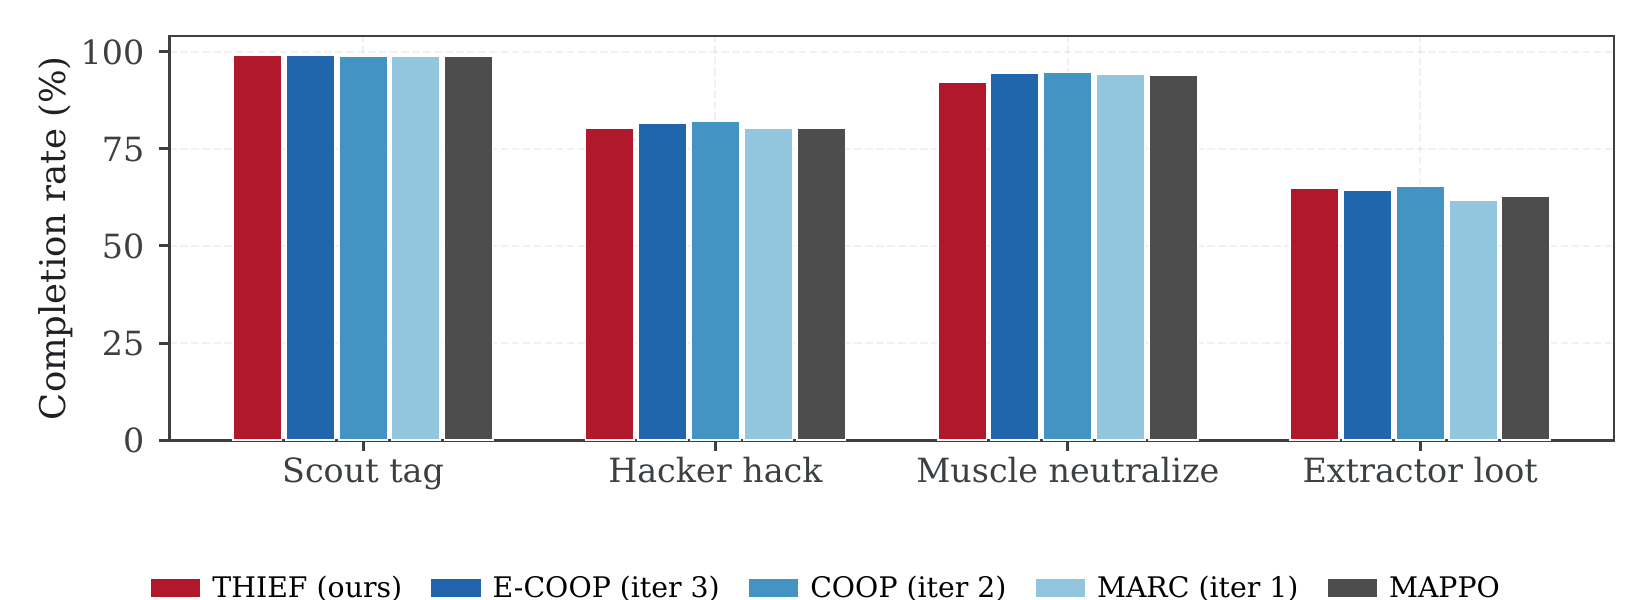
\includegraphics[width=\linewidth]{figures/stage3_subtasks.pdf}
\caption{\textbf{Role Subtask Success Rates on Stage 3.} Grouped bar breakdown of role-specific subtask completion for the method lineage (MARC, COOP, E-COOP, THIEF) against the leading external baseline (MAPPO), evaluated over $N=1,\!000$ episodes across 10 random training seeds ($10,\!000$ episodes per algorithm).}
\label{fig:subtasks}
\end{figure}

% Auto-generated by paper/scripts/generate_tables.py. Do not edit manually.
\begin{table}[htbp]
\centering
\caption{Role subtask completion rates and tactical telemetry on Stage 3 ($35\times 35$, 3 guards, 2 cameras, 3 locked doors). Evaluation over $N=1,\!000$ episodes across 10 random seeds ($10,\!000$ episodes total per algorithm). Partitioned into our iterative development lineage versus external baselines. Bold denotes highest completion rate or lowest alarm overall.}
\label{tab:subtasks_stage3}
\vspace{0.04in}
\footnotesize
\setlength{\tabcolsep}{2.5pt}
\renewcommand{\arraystretch}{1.06}
\begin{tabular}{l ccccc cc}
\toprule
\textbf{Method} & \textbf{Scout} & \textbf{Hacker} & \textbf{Muscle} & \textbf{Extractor} & \textbf{Agents} & \textbf{Mean} & \textbf{Mean} \\
 & \textbf{Tag (\%)} & \textbf{Hack (\%)} & \textbf{Neut. (\%)} & \textbf{Loot (\%)} & \textbf{Extracted} & \textbf{Alarm} & \textbf{Steps} \\
\midrule
\multicolumn{8}{l}{\textit{\textbf{Proposed Method Lineage (Ours)}}} \\
\midrule
\textbf{THIEF (Ours, Final)} & \textbf{99.1\%} & 80.3\% & 92.2\% & 65.0\% & 2.37 & 89.1 & 775.3 \\
E-COOP (Iteration 3) & 99.0\% & 81.5\% & 94.5\% & 63.9\% & 2.46 & 86.8 & 859.3 \\
COOP (Iteration 2) & 98.8\% & 81.9\% & \textbf{94.7\%} & \textbf{65.3\%} & \textbf{2.49} & 87.5 & 851.4 \\
MARC (Iteration 1) & 98.8\% & 80.4\% & 94.1\% & 61.8\% & 2.37 & 89.3 & 895.4 \\
\midrule
\multicolumn{8}{l}{\textit{\textbf{External MARL Baselines}}} \\
\midrule
ROMA \cite{wang2020roma} & 99.0\% & \textbf{82.6\%} & 94.5\% & 65.2\% & 2.47 & 89.0 & 863.6 \\
RODE \cite{wang2021rode} & 98.7\% & 78.3\% & 94.0\% & 59.5\% & 2.24 & 98.8 & 913.0 \\
MAPPO \cite{yu2022surprising} & 98.8\% & 80.5\% & 94.0\% & 62.6\% & 2.39 & 89.4 & 889.1 \\
H-MAPPO \cite{vezhnevets2017feudal} & 96.6\% & 40.5\% & 92.8\% & 21.4\% & 0.86 & \textbf{86.6} & 1307.1 \\
COMA \cite{foerster2018counterfactual} & 98.7\% & 74.0\% & 93.5\% & 55.6\% & 2.03 & 92.8 & 985.5 \\
\bottomrule
\end{tabular}
\end{table}


\section{Component Micro-Ablations of THIEF}
\label{sec:app_ablation}
To isolate the contribution of each core mechanism, we evaluate THIEF standalone (fresh initialization, identical per-stage budgets and hyperparameters) on two diagnostic stages: Stage 2 ($25 \times 25$), where expert spawning is actively triggered across training, and Stage 4 ($50 \times 50$), the long-horizon regime in which final claims are evaluated. Results are evaluated over $1,\!000$ held-out episodes per seed across random training seeds (Table~\ref{tab:ablations}).

The ablated variants are:
\begin{itemize}[leftmargin=*,nosep]
    \item \textbf{w/o warmup} ($\tau_{\text{iso}}=0$): newly spawned specialists skip isolated sandbox environments and join the global bidding pool immediately with uncalibrated critics.
    \item \textbf{w/o Fisher geometry}: parent recombination uses uniform parameter averaging with isotropic noise, removing curvature weighting and inverse-Fisher exploration scaling.
    \item \textbf{clone-best-parent}: the specialist actor is a perturbed copy of the best parent (no pool recombination, no deficit gradient push), isolating recombination from single-parent cloning.
    \item \textbf{w/o load balancing} ($\alpha_{\text{bal}}=0$): the load-balancing regularizer of Section~\ref{sec:thief} is removed.
    \item \textbf{w/o hysteresis} ($\epsilon=0$): the routing barrier is disabled, allowing unconstrained per-step switching.
    \item \textbf{fixed-schedule spawning}: the win-rate plateau trigger is bypassed in favor of spawning on a fixed update cadence.
\end{itemize}
All variants are trained and evaluated with identical per-stage budgets and hold-out protocols. The first four rows (full THIEF, w/o warmup, w/o Fisher geometry, clone-best-parent) aggregate 10 random seeds per stage; the w/o load balancing, w/o hysteresis, and fixed-schedule variants use a 3-seed diagnostic budget (seeds 0--2), so their standard errors are correspondingly larger and no cross-variant significance is claimed for them.

\InputIfFileExists{tables/ablation}{}{}

\section{Environment Implementation \& Engineering Details}
\label{sec:app_env}
The HEIST simulation engine is developed in native Rust to eliminate Python GIL bottlenecks during multi-agent pathfinding and raytraced field-of-view perception:
\begin{itemize}[leftmargin=*,nosep]
    \item \textbf{Raytraced Line of Sight:} For each agent coordinate, ray traversal is computed along 8 cardinal and diagonal directions. Rays terminate upon encountering perimeter or interior room walls, populating visible tiles into egocentric observation arrays with value $-1$ for occluded fog-of-war tiles.
    \item \textbf{Adversarial Guard Pathfinding:} Guard pathfinding uses a breadth-first search (BFS) queue executed over cached grid obstacle bitmasks. Guard investigation states pathfind toward the last-known coordinate of spotted agents.
    \item \textbf{Zero-Copy PyTorch Sharding:} Simulation steps execute across parallel environments using Rayon worker threads. Observations, rewards, done flags, and action masks are copied directly into pre-allocated contiguous CUDA/CPU tensors.
\end{itemize}

\section{Full Hyperparameter Specifications}
\label{sec:app_hyperparameters}
Table~\ref{tab:hyperparameters} provides the universal hyperparameters shared across all algorithms. The centralized critic input dimensionality of $2,\!550 + 4 + 2$ decomposes as: $6$ global scalars (step counter, alarm, terminal/loot/extraction flags, extraction countdown) $+\; 50 \times 50 = 2,\!500$ grid cells $+\; 8$ agent coordinates $+\; 12 \times 2 = 24$ guard coordinates (unused guard slots padded with $-1$) $+\; 12$ guard-neutralization flags $= 2,\!550$, plus the $4$-dimensional role embedding and $2$-dimensional mission compass. Because the $50 \times 50$ grid canvas and the 12 guard slots are fixed capacity across all curriculum stages (cells outside the active stage's floorplan hold the wall token), this input dimensionality is identical at every stage, which is precisely what allows critic checkpoints to transfer between curriculum stages without architectural modification.

% Universal training and architectural hyperparameters.
\begin{table}[t]
\centering
\caption{Universal training and architectural hyperparameters across all evaluated MARL algorithms (verified against the reference implementation). Environment- and algorithm-specific values are noted where they differ.}
\label{tab:hyperparameters}
\vspace{0.06in}
\small
\setlength{\tabcolsep}{4.0pt}
\renewcommand{\arraystretch}{1.08}
\begin{tabular}{ll}
\toprule
\textbf{Hyperparameter} & \textbf{Value} \\
\midrule
Actor Network Architecture & 2-layer MLP ($[49+4+2] \rightarrow 64 \rightarrow 64 \rightarrow 6$), Tanh \\
Critic Network Architecture & 2-layer MLP ($[2,\!550+4+2] \rightarrow 64 \rightarrow 64 \rightarrow 1$), Tanh \\
Optimizer & Adam ($\text{lr} = 2.5 \times 10^{-4}$, $\epsilon = 10^{-5}$) \\
PPO Clip Ratio ($\epsilon_{\text{clip}}$) & 0.20 \\
Discount Factor ($\gamma$) & 0.99 \\
GAE Parameter ($\lambda_{\text{gae}}$) & 0.95 \\
PPO Epochs per Update & 4 \\
Mini-batches per Update & 4 (batch size / 4) \\
Entropy / Value Coefficients & 0.01 / 0.5 \\
Rollout Horizon ($T$) & 125 steps (all stages) \\
Vectorized Environments & 16 (THIEF, E-COOP); 8 (all other methods) \\
Updates per Stage & 100/100/250/450/800 (16 envs); $2\times$ for 8-env baselines \\
Training Budget per Stage & $2/2/5/9/16 \times 10^5$ env.\ steps (Stages 0--4) \\
\midrule
\multicolumn{2}{l}{\emph{THIEF-specific}} \\
Hysteresis Barrier ($\epsilon$) & 0.05 \\
Plateau Trigger ($\Delta_{\text{win}}$) & $< 0.03$ over last 100 episodes ($\ge 200$ recorded) \\
Spawning Ceiling & suppressed when recent win rate $\ge 0.90$ \\
Incubation Duration ($\tau_{\text{iso}}$) & 10 updates (4 of 16 environments, 25\%) \\
Fisher Decay ($\beta$) & 0.99 \\
Mutation Noise Scale & 0.03 \\
Targeted Deficit Learning Rate ($\eta_{\text{def}}$) & 0.08 \\
Load-Balancing Coefficient ($\alpha_{\text{bal}}$) & 0.01 \\
Dormancy Cull Window ($\tau_{\text{cull}}$) & $\max(60,\, 0.4\,T_{\text{upd}})$ zero-usage updates \\
\bottomrule
\end{tabular}
\end{table}

\paragraph{Hyperparameter Grouping and Sensibility.}
THIEF introduces interdependent hyperparameters beyond the shared PPO backbone; they fall into four mechanism families (all values in Table~\ref{tab:hyperparameters} are held fixed across every seed, stage, and algorithm comparison in this paper): (i) \emph{plateau triggering} --- window $W=100$, threshold $\Delta_{\text{win}}<0.03$, mastery ceiling $0.90$; (ii) \emph{incubation} --- $\tau_{\text{iso}}=10$ updates over a dedicated $25\%$ environment fraction; (iii) \emph{Fisher geometry} --- EMA decay $\beta=0.99$, damping $\lambda=10^{-4}$, deficit step size $\eta_{\text{def}}=0.08$, noise scale $\sigma=0.03$; and (iv) \emph{routing} --- barrier $\epsilon=0.05$, gating temperature $\tau_{\text{gate}}$, balance coefficient $\alpha_{\text{bal}}=0.01$, dormancy threshold $\tau_{\text{cull}}$. Families (ii)--(iv) are exercised in isolation by the micro-ablations of Table~\ref{tab:ablations} (w/o warmup, w/o Fisher geometry, clone-best-parent, w/o load balancing, w/o hysteresis), which probe the qualitative sensitivity of end-to-end performance to removing each mechanism outright; the full THIEF variant degrades gracefully across all of them. We did not run exhaustive per-threshold sweeps (e.g., $\epsilon \in [0.01, 0.10]$ or $\Delta_{\text{win}} \in [0.03, 0.05]$) and flag complete sensitivity analysis as future work.

\section{Compute Environment \& Hardware Throughput}
\label{sec:app_compute}
All benchmark training and evaluation runs were conducted on a single Linux workstation equipped with an NVIDIA GeForce RTX 3080 Ti GPU (12 GB VRAM) and an AMD Ryzen 9 5900X 12-core processor (24 threads). The raw Rust simulation engine sustains approximately $11,\!500$--$12,\!500$ environment steps per second across the curriculum stages (measured over $N=1,\!000$-episode evaluation batches for single-network policies such as MAPPO, MARC, and COMA); end-to-end throughput for multi-expert methods is lower due to per-expert forward passes (e.g., approximately $2,\!400$--$3,\!200$ steps/s for THIEF). Each curriculum stage trains for a fixed budget of $2/2/5/9/16 \times 10^{5}$ environment steps (Stages 0--4, $3.4 \times 10^6$ per seed in total), corresponding to 100/100/250/450/800 PPO updates across all evaluated models using 16 parallel environments uniformly ($16 \times 125 = 2,\!000$ steps per rollout).


\end{document}